\documentclass{sig-alternate}
\usepackage{graphicx}
\usepackage{listings}
\usepackage{xcolor}
\lstset{language=Matlab}
\lstset{
	backgroundcolor=\color{gray!5},
	rulecolor=\color{gray!10},
	basicstyle=\ttfamily,
	keywordstyle=\color{blue}\bf\it,
	commentstyle=\it\color[RGB]{0,96,96},
	stringstyle=\rmfamily\slshape\color[RGB]{64,128,128},
}
\lstset{breaklines}
\lstset{extendedchars=false}
\begin{document}
\title{Homework 3 Linear Regression: Experiment \\\begin{it} CSE 847: Machine Learning	\end{it}}
\author{Nan Cao}
\maketitle
\begin{bf} Question1:\end{bf}
$$f(\omega)=\frac{1}{2}{||X\omega-y||}_2^2+\frac{\lambda}{2}{||\omega||}_2^2$$
$$f'(\omega)=X^TX-X^Ty+\lambda\omega$$
$$Let f'(\omega)=0$$
$$X^TX\omega-X^Ty+\lambda\omega=0$$
$${\hat{\omega}}_{Ridge}=\frac{X^Ty}{\lambda I+X^TX}$$  
The following function is used to compute the ${\hat{\omega}}_{Ridge}$ with the given x and y.
\begin{lstlisting}
function [ w ] = RidgeReg( x, y, Lamda )
	X2 = x' * x;
	[n1, n2] = size(X2);
	a = Lamda * (eye(n1, n2))+X2;
	if det(a) == 0
		display('singular matrix, unable to implement the ridge regression');
	else
		w = a^(-1)* (x' * y);
end
\end{lstlisting}  
\begin{bf} Question2:\end{bf}
The following function is used to compute the MSE with the given ${\hat{\omega}}_{Ridge}$ x and y.
\begin{lstlisting}
function [ MSE ] = MSE( w, x, y )
	a=x * w - y;
	N = length(y);
	MSE = (1/N) * ((norm(a,2))^2);
end
\end{lstlisting}
The follow codes are used to compute the MSEof different $\lambda$ and plot them in the same figure.
\begin{lstlisting}
LamdaError = zeros(3, 7);
LamdaError(1,1:7) = [1e-5, 1e-4, 1e-3, 1e-2, 1e-1, 1, 10];
for i=1 : 1 : 7
	w1=RidgeReg(x_train, y_train,LamdaError(1, i));
	LamdaError(2, i)=MSE(w1, x_train, y_train);
	LamdaError(3, i)=MSE(w1, x_test, y_test);
end
LogScale = log (LamdaError(1,1:7));
LamdaError
plot(LogScale, LamdaError(2,1:7),'k.',LogScale, LamdaError(3,1:7),'kp');
\end{lstlisting}
Following are the output results of both training and testing dataset
\begin{verbatim}
LamdaError =

1.0e+04 *

0.0000 0.0000 0.0000 0.0000 0.0000 0.0001 0.0010
1.9695 2.0060 2.0385 2.0919 2.2076 2.4731 2.7165
7.691  5.7532 4.9061 4.4405 3.6995 3.0518 3.0057
\end{verbatim}
The plot of MSE of training and testing data under different $\lambda$\\
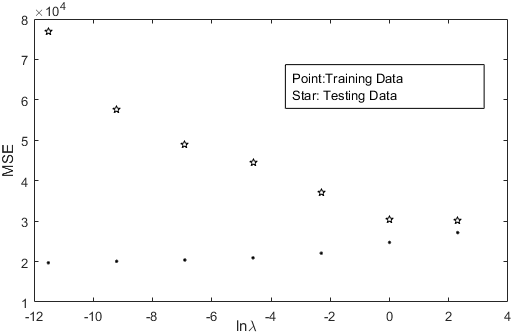
\includegraphics [width=3in,height=2in] {errorcompare.png} \\
\begin{bf} Question3:\end{bf}
To perform 5-fold cross validation
\begin{lstlisting}
Lamda(1:7) = [1e-5, 1e-4, 1e-3, 1e-2, 1e-1, 1, 10]
for i=1 : 1 : 7
	for k=1 : 1 : 5
		KFC_testX=x_train(2+48*(k-1):1+48*k,1:64)
		KFC_testY=y_train(2+48*(k-1):1+48*k,1)
		KFC_trainX(1:194,1:64)=x_train([1:1+48*(k-1),2+48*k:242],1:64)
		KFC_trainY=y_train([1:1+48*(k-1),2+48*k:242])
		KFC_w=RidgeReg(KFC_trainX, KFC_trainY, Lamda(i))
		KFC_MSE(k)=MSE(KFC_w, KFC_testX, KFC_testY)
	end
	Lam_MSE(i)=mean(KFC_MSE)
end
Lam_MSE
\end{lstlisting}
\begin{verbatim}
Lam_MSE =

1.0e+05 *

1.2870 0.9394  0.6376 0.4533 0.3369 0.2889 0.2801
\end{verbatim}
It shows that the best $\lambda$ for estimated from the training data is 10
\end{document}